\documentclass{scrartcl}

\usepackage[T1]{fontenc}
\usepackage[utf8]{inputenc}

\title{Mobile Dev A3.3C}
\author{Daniel Coady (102084174)}
\date{23/09/2019}

\usepackage{graphicx}

\begin{document}

\maketitle

\section*{Part 1}
In this application there are two different fragments:
\begin{itemize}
    \item The single date view for each location in the view pager
    \item The date views in the generate table activity for the recycler view
\end{itemize}

\begin{figure}[h]
    \centering
    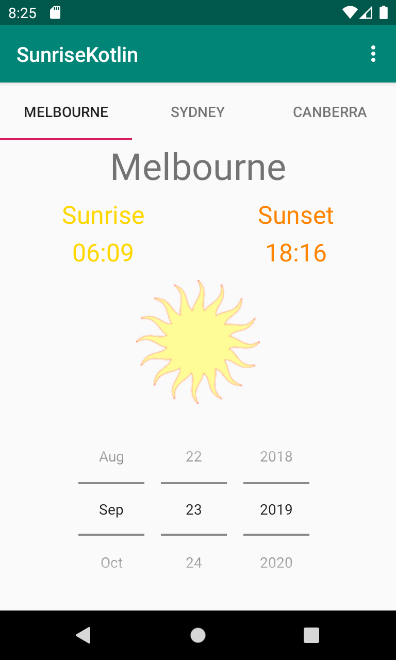
\includegraphics[scale=0.5]{images/screen1.png}
    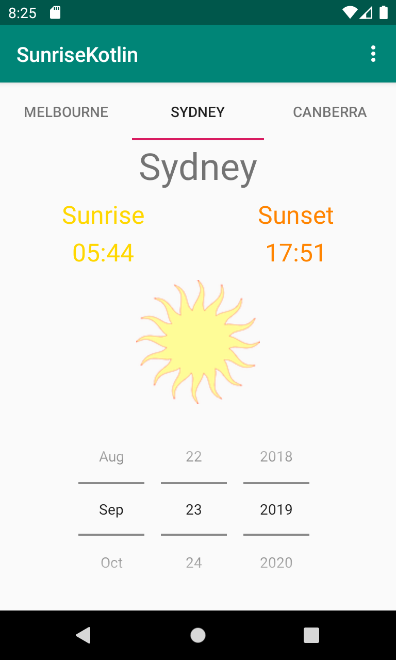
\includegraphics[scale=0.5]{images/screen2.png}
    \caption{The screen that will appear as you launch the application and viewing another location}
\end{figure}

\pagebreak

\begin{figure}[h]
    \centering
    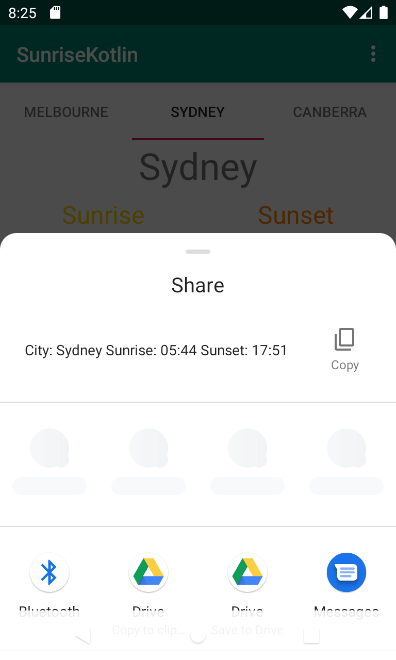
\includegraphics[scale=0.5]{images/screen3.png}
    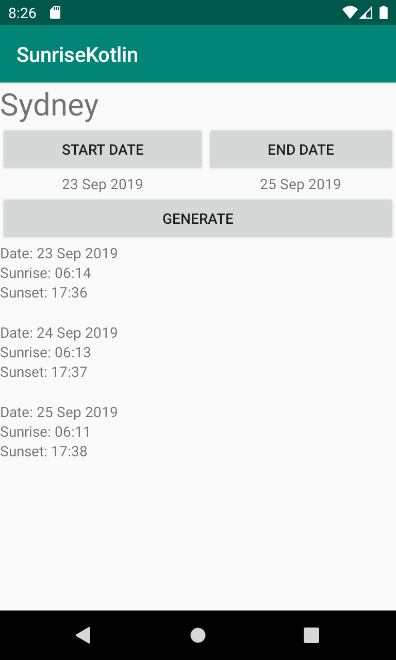
\includegraphics[scale=0.5]{images/screen4.png}
    \caption{Share and generate table functionality}
\end{figure}

\begin{figure}[h]
    \centering
    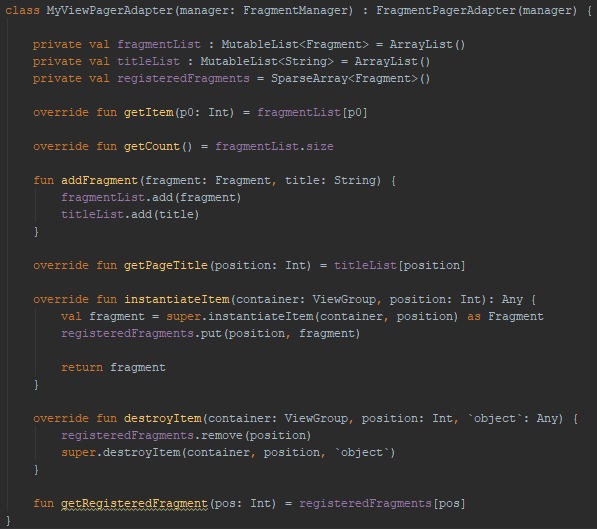
\includegraphics[scale=0.8]{images/screen5.png}
    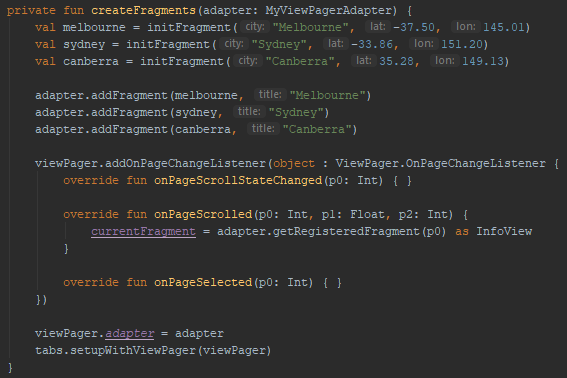
\includegraphics[scale=0.8]{images/screen6.png}
    \caption{Code related to the fragments in the main activity}
\end{figure}

\begin{figure}[h]
    \centering
    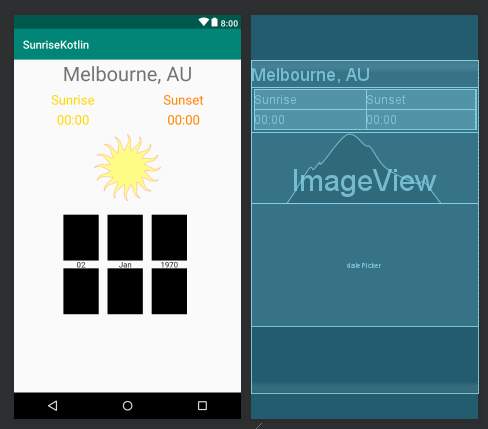
\includegraphics{images/screen7.png}
    \caption{Fragment used in the main activity}
\end{figure}

\end{document}
